\section{Literature Review}
\label{sec:litreview}

You can mention previous chapters, like Chapter \ref{sec:introduction}, using the label that you have written before.

\subsection{\textbf{Add the title of your subsection here}}
\label{sec:labelname}

\vspace{0.1 in}
\noindent
You can also add labels to a subsection, like in \ref{sec:labelname}




\vspace{0.1 in}
\noindent


Let's add one equation that you can cite in your text \ref{eq:name_of_your_equation}

\vspace{0.1 in}
\noindent

\begin{equation}
\label{eq:name_of_your_equation}
y = mx + n
\end{equation}


\vspace{0.1 in}
\noindent

Let's add a table that you can reference in the text too, Table \ref{table:myparameters}. I prefer to add tables as figures, but they can also be created in the visual editor or with some latex code in the code editor.

\begin{table}[H] %  figure placement: here, top, bottom, or page
    \centering
    \caption{Parameters that I use in my experiments}
    \label{table:myparameters}    
    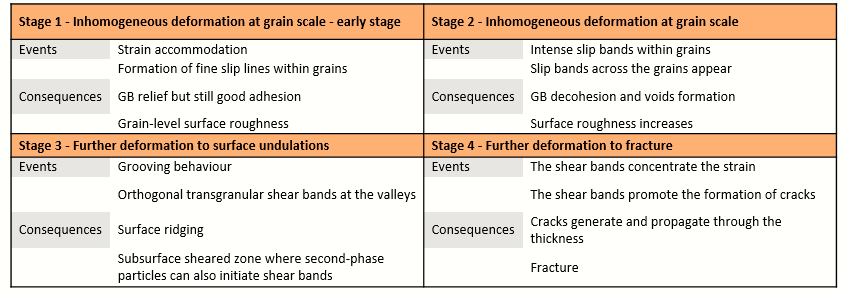
\includegraphics[width=6in]{Figures/LitRev/Stages_table_title.png}
\end{table}

\vspace{0.1 in}
\noindent
You can add Figures too, like in Figure \ref{fig:imagelabel}. 

\begin{figure}[H] %  figure placement: here, top, bottom, or page
    \centering
    
\includegraphics[width=3.5in]{Figures/LitRev/image.png}
    \caption{photo}
    \label{fig:imagelabel}
\end{figure}
